\documentclass{report}
\usepackage[utf8]{inputenc}
\usepackage{amsmath}
\usepackage{amsfonts}
\usepackage{hyperref}
\usepackage{tcolorbox}
\usepackage{breqn}
\usepackage{adjustbox}
\usepackage{changepage}
\usepackage{rotating}
\usepackage{algorithm}
\usepackage{algpseudocode}
\usepackage{ntheorem}
\usepackage{subcaption}

% Definition
\newtheorem{definition}{Definition}{\bfseries}{\itshape}
\newtheorem*{definition*}{Definition}{\bfseries}{\itshape}

% Theorem
\newtheorem{theorem}{Theorem}{\bfseries}{\itshape}

% Concept
\newtheorem*{concept}{}{\bfseries}{\itshape}

\title{Analysis of diffusion in the DES cipher}
\author{Ana Clara Zoppi Serpa\\ Prof. Dr. Ricardo Dahab \\ Dr. Jorge Nakahara Jr.}
\date{\today}

\begin{document}

\maketitle

\tableofcontents

\chapter{Analysis of diffusion in the DES cipher}

% Listar as coisas que já são conhecidas de capítulos anteriores
% Informar o propósito do capítulo

In this chapter, we analyze complete diffusion in the DES cipher \cite{DES-FIPS} with regards to plaintext and key. Both plaintext and key diffusion are complete after the $5$-th round. The analysis is performed using a graph (see Section \ref{sec:prelim}) to model the dependencies between plaintext/key bits and round output (state) bits.

We assume the reader is familiar with:
\begin{itemize}
    \item the DES $S$-Box diffusion analysis conducted in \textcolor{red}{Chapter X},
    \item the DES cipher (expansion $E$, $S$-boxes, bit permutation $P$, Feistel Network structure).
\end{itemize}

\section{Notation}
\begin{itemize}
    \item $G$: a graph
    \item $V$: set of vertices of a graph
    \item $E$: set of edges of a graph
    \item $|V|, |E|$: cardinality (number of elements of) the sets $V$ and $E$, respectively
    \item $A[i][j]$: element at row $i$, column $j$ of the matrix $A$
    \item $\mathcal{A}$: adjacency-list representation of a graph
    \item $\mathcal{A}[v]$: adjacency list for the vertex $v$ of a graph
    \item $x^j_i$: $i$-th state bit after round $j$ of DES (note that, if $j = 0$, it is a plaintext bit)
    \item $L_j$: left half of DES state after $j$-th round, comprising bits from $x^j_1$ to $x^j_{32}$
    \item $R_j$: right half of DES state after $j$-th round, comprising bits from $x^j_{33}$ to $x^j_{64}$
    \item $F$: application of the DES $F$ function
    \item $K_j$: $j$-th subkey of DES, used at the $j$-th round, containing 48 bits
    \item $E$: the expansion function $E$ of DES
    \item $P$: the bit permutation $P$ of DES
    \item $P[i]$: result of applying the DES permutation $P$ to $i$ ($i$ ranges from 1 to 64)
    \item $i_t$: $t$-th input bit of an $S$-Box
    \item $e_t$: $t$-th input bit of the expansion function $E$
    \item $S_1$, $S_2$, ..., $S_8$: DES $S$-Boxes
    \item $s^j_i$: output bit of an $S$-Box, $i$ is the bit position with respect to the DES state (from 1 to 64), $j$ is the round (from 1 to 16)
    \item $PC1$, $PC2$: permutations used in the DES key schedule
    \item $C_i, D_i, B$: intermediate variables in the DES key scheduling algorithm
    \item $K_{j,z}$: $z$-th bit of the $r$-th round subkey of DES
    \item $k_p$: $p$-th bit of the DES master key
\end{itemize}

\section{Acronyms}
\begin{itemize}
    \item DES: Data Encryption Standard
    \item ANF: Algebraic Normal Form
    \item $S$-Box: Substitution Box
\end{itemize}

\section{Preliminaries}\label{sec:prelim}
% Colocar conceitos de grafos aqui
% Nós e arestas
% Caminho
% Matriz de adjacência
% Lista de adjacência

\begin{concept}[Graph]
A graph $G = (V, E)$ is a set of vertices (also called nodes) $V$ together with a set of edges $E$ that connect vertices. Each edge is a tuple $(v_1, v_2)$, meaning that vertices $v_1$ and $v_2$ are connected.
\end{concept}

\begin{concept}[Adjacency matrix representation of a graph]
In an adjacency matrix representation, we assume the vertices of the graph $G = (V, E)$ are numbered, for instance, from $1$ to $|V|$. The $|V| \times |V|$ matrix $A$ such that $A[v_1][v_2] = 1$ if $(v_1, v_2) \in E$ (0 otherwise) is the adjacency matrix of the graph. In other words, it is a matrix where $1$ means the vertices given by the row and the column are connected and $0$ means they are not connected.
\end{concept}

\begin{concept}[Adjacency-list representation of a graph]
The adjacency-list representation consists of an array of $\mathcal{A}$ of $|V|$ lists, one for each vertex. For each $v \in V$, the list $\mathcal{A}[v]$ contains all vertices $u$ such that $(v, u) \in E$, i.e all the vertices to which $v$ is connected.
\end{concept}

When two vertices are connected, we say they are \emph{adjacent}, or that they are \emph{neighbors}. For the plaintext diffusion analysis, we take advantage of the adjacency matrix representation. For the key diffusion analysis, we use adjacency lists.

Furthermore, two vertices $v_1$ and $v_2$ might not be directly connected to each other by an $(v_1, v_2)$ edge, but there might exist a \emph{path} from one to the other. There is a path from $v_1$ to $v_2$ if it is possible to reach $v_2$ from $v_1$. For example, if we have edges $(v_1, v_3)$ and $(v_3, v_2)$, $v_1$ and $v_2$ are not directly connected by an edge, but we can reach $v_2$ by going from $v_1$ to $v_3$ and then from $v_3$ to $v_2$. Therefore, there is a path from $v_1$ to $v_2$.

For the purposes of the analysis conducted in this chapter, these concepts are sufficient. However, for more details about graphs, algorithms and problems related to this data structure, the reader can refer to \cite{Cormen2009}.

The core idea in order to analyze diffusion for the DES cipher is to represent each state bit at each round as a node (vertex) in a graph and use edges (and paths) to represent dependence between them and plaintext (or key) bits.

\section{Plaintext diffusion}

Let $x_i^j$ denote the $i$-th state bit after round $j$ of DES. At any given round $j$, we have $x_1^j, x_2^j, ..., x_{64}^j$, which is input to round $j + 1$. For each state bit, a node is created on a graph, and edges track dependence between them. In this way, we can track how many plaintext bits, i.e bits with $j = 0$, influence other bits throughout the rounds of DES.

The DES transformations occur as follows.

\begin{equation*}
    L_j = R_{j-1},
\end{equation*}

\begin{equation*}
    R_j = L_{j-1} \oplus F(R_{j-1}, K_j).
\end{equation*}

For iteration 1, for instance,

\begin{equation*}
    L_1 = R_0,
\end{equation*}

\begin{equation*}
    R_1 = L_{0} \oplus F(R_{0}, K_0).
\end{equation*}

Before any of the transformations take place, the plaintext is $x_1^0, x_2^0, x_3^0, ..., x_{64}^0$, where the left half ($L_0$) comprises the bits from $x_1^0$ to $x_{32}^0$ and the right half ($R_0$) starts at $x_{33}^0$ and ends at $x_{64}^0$.

For round $1$, the right half of round $0$ is copied to become the left half ($L_1 = R_0$), thus we create edges between nodes $x_1^1$ and $x_{33}^0$, between $x_2^1$ and $x_{34}^0$, and so forth, respectively, with the edge between $x_{32}^1$ and $x_{64}^0$ being the last one created to represent the dependence incurred by the $L_1 = R_0$ step. Figure \ref{fig:feistel-step-1} shows the nodes and edges related to this process. White nodes are plaintext nodes, red nodes are round $1$ nodes.

\begin{figure}[h!]
    \centering
    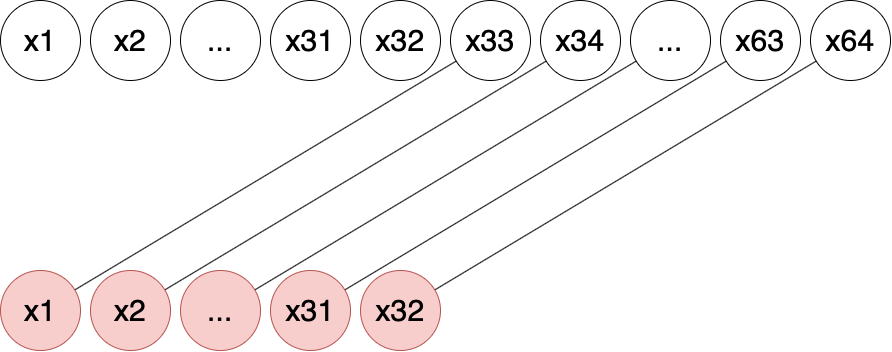
\includegraphics[scale=0.3]{Grafo_DES-L1equalsR0.png}
    \caption{Diffusion incurred by $L_1 = R_0$. Each bit of the left half depends on a corresponding bit on the right half of the plaintext.}
    \label{fig:feistel-step-1}
\end{figure}

Regarding $R_1 = L_0 \oplus F(R_0, K_0)$, there is dependence between bits of $R_1$ and bits of $L_0$, thus we need edges between $x_{33}^1$ and $x_1^0$, between $x_{34}^1$ and $x_2^0$, and so forth, respectively, with the edge between $x_{64}^1$ and $x_{32}^0$ being the last. Figure \ref{fig:feistel-step-2} illustrates this. 

\begin{figure}[h!]
    \centering
    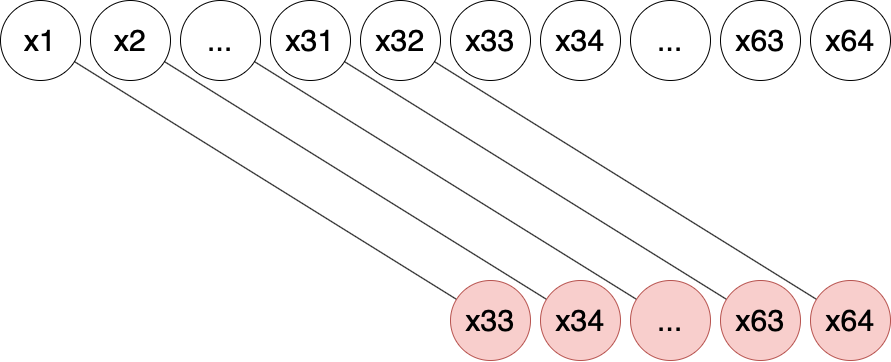
\includegraphics[scale=0.3]{Grafo_DES-R1equalsL0XOR.png}
    \caption{Diffusion incurred by the XOR with $L_0$ when $R_1 = L_0 \oplus F(R_0, K_0)$. Each bit of the right half depends on the corresponding bit on the left half of the plaintext.}
    \label{fig:feistel-step-2}
\end{figure}

\begin{figure}[h!]
    \centering
    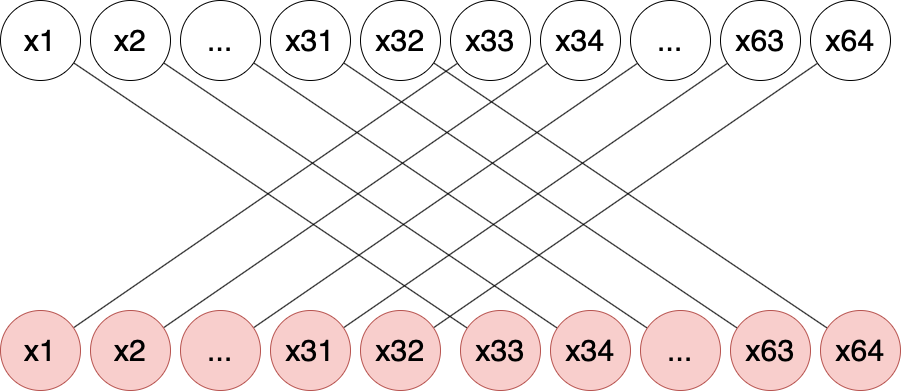
\includegraphics[scale=0.3]{Grafo_DES-halves-trivial.png}
    \caption{Diffusion incurred by $R_1 = L_0$ and by the XOR with $L_0$ when $R_1 = L_0 \oplus F(R_0, K_0)$, shown together}
    \label{fig:feistel-xors-together}
\end{figure}

These edges keep track of the dependence caused by the XOR function and the Feistel structure only (see Figure \ref{fig:feistel-xors-together}). In order to analyze how the $F$ function provides diffusion, we must consider each step of it: the expansion function $E$, the $S$-boxes, and the permutation $P$. Furthermore, for the moment, we ignore the key, assuming each $K_i = 0$, so that we can focus only on plaintext diffusion. Key diffusion is addressed in Section \ref{sec:key-diff}.

\subsection{The $S$-boxes}
From the $S$-Box analysis conducted with the ANFs in \textcolor{red}{Chapter X}, we know that each $S$-box takes $6$ input bits and completely diffuses them over the $4$ output bits. Therefore, if $i_1, i_2, i_3, i_4, i_5, i_6$ are the inputs to an $S$-box and $y_1, y_2, y_3, y_4$ are the outputs, each $y_j$  depends on all of the $i_t$, for $1 \leq j \leq 4$ and $1 \leq t \leq 6$, since the $S$-box achieves complete diffusion.

\subsection{The $E$ expansion function}
Given $32$ input bits $e_1, e_2, e_3, ..., e_{32}$, the $E$ function expands them to $48$ bits. This is done by appending repeated bits to the left and to the right of each $4$-bit slice, according to Table \ref{tab:expansion}. For the first slice, from $e_1$ to $e_4$, $e_{32}$ is appended to the left and $e_5$ is appended to the right. For the second slice, $e_4$ is appended to the left and $e_9$ is appended to the right, and so forth. For the last slice, $e_{28}$ is appended to the left and $e_{1}$ is appended to the right. The output is thus $e_{32}, e_1, e_2, e_3, e_4, e_5, e_4, e_5, e_6, e_7, e_8, e_9, e_8, e_9, ..., e_{30}, e_{31}, e_{32}, e_1$. 

In general, for each $4$-bit slice of the original input starting at $e_k$ and ending at $e_p$, $e_{p+1}$ is appended to the right, and $e_{k-1}$ is appended to the left. If $p+1 = 33$, then $e_1$ is appended. If $k-1 = 0$, then $e_{32}$ is appended.

\begin{table}[h!]
\centering
\begin{tabular}{|c|c|c|c|c|c|}
\hline
\multicolumn{6}{|c|}{E}                                         \\ \hline
32 & \textbf{1}  & \textbf{2}  & \textbf{3}  & \textbf{4}  & 5  \\ \hline
4  & \textbf{5}  & \textbf{6}  & \textbf{7}  & \textbf{8}  & 9  \\ \hline
8  & \textbf{9}  & \textbf{10} & \textbf{11} & \textbf{12} & 13 \\ \hline
12 & \textbf{13} & \textbf{14} & \textbf{15} & \textbf{16} & 17 \\ \hline
16 & \textbf{17} & \textbf{18} & \textbf{19} & \textbf{20} & 21 \\ \hline
20 & \textbf{21} & \textbf{22} & \textbf{23} & \textbf{24} & 25 \\ \hline
24 & \textbf{25} & \textbf{26} & \textbf{27} & \textbf{28} & 29 \\ \hline
28 & \textbf{29} & \textbf{30} & \textbf{31} & \textbf{32} & 1  \\ \hline
\end{tabular}
\caption{The DES expansion function}
\label{tab:expansion}
\end{table}

For the first round of DES, $R_0$ is the input to the expansion function $E$, thus bits from $x_{33}$ to $x_{64}$ are expanded.

\subsection{Expansion function and S-box}
After the expansion, these bits are fed into the $S$-boxes. $S$-box $S_1$ gets $x_{33}^0, x_{34}^0, x_{35}^0$ and $x_{36}^0$ as its input, i.e, the first $4$-bit slice of the right half, and also $x_{64}^0$ and $x_{37}^0$, according to the expansion $E$. $S_2$ gets $x_{37}^0, x_{38}^0, x_{39}^0, x_{40}^0$ (the second slice), and also $x_{36}$ and $x_{41}$, because of the expansion function. In general, each $S$-box gets the current $4$-bit slice bits as input plus the two extension bits.

If we denote $S$-box output bits by $s_i^j$, where $i$ is the bit position at the state and $j$ is the round, we can use the ANFs to track dependencies between $s_i^1$ and plaintext bits. If a bit shows up at the ANF, an edge should be created for it in the graph. There should thus be edges between $s_{33}^1$ and $x_{33}^0, x_{34}^0, x_{35}^0, x_{36}^0, x_{64}^0$ and $x_{37}^0$. There should be edges between $s_{34}$ and $x_{33}^0, x_{34}^0, x_{35}^0, x_{36}^0, x_{64}^0$ and $x_{37}^0$, and so forth. For each $s_i^1$, for $i$ between $33$ and $64$, similar analysis applies, since the ANFs completely diffuse the input bits. Figures \ref{fig:expansion1} to \ref{fig:expansion4} illustrate this.

\begin{figure}[h!]
    \centering
    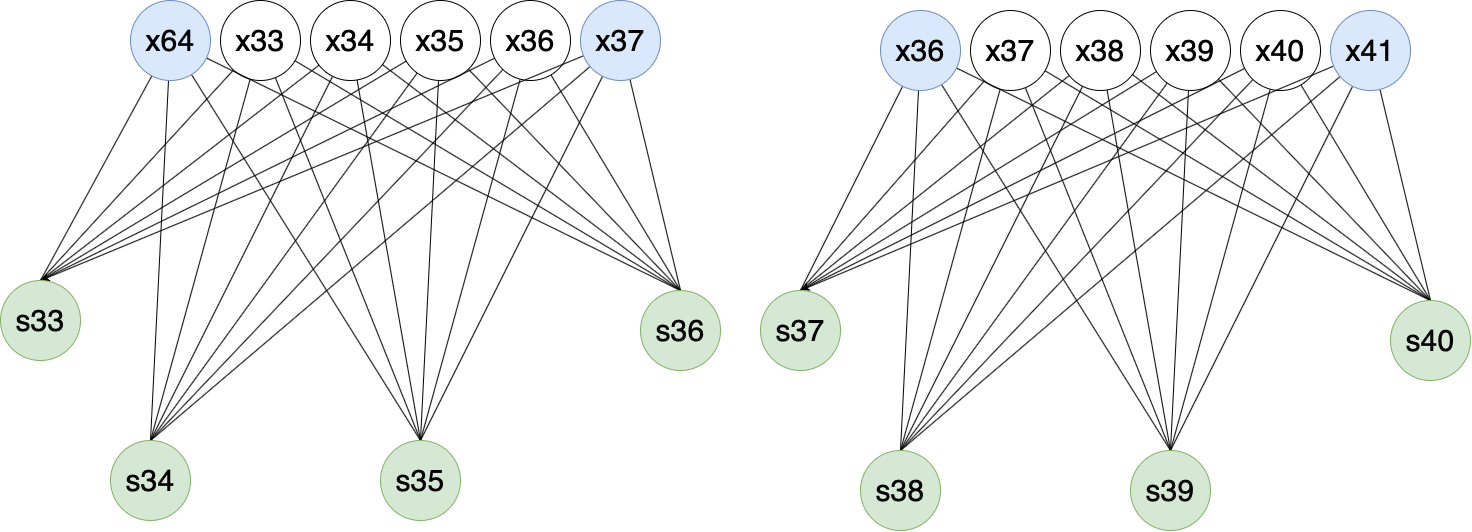
\includegraphics[scale=0.3]{Grafo_DES-Expansion1.png}
    \caption{Graph edges for expansion function and $S$-box ($S_1$ and $S_2$) analysis. Each $S$-box output depends on all the six input bits, which are the plaintext bits of the current slice being considered plus the expansion function bits (blue).}
    \label{fig:expansion1}
\end{figure}

\begin{figure}[h!]
    \centering
    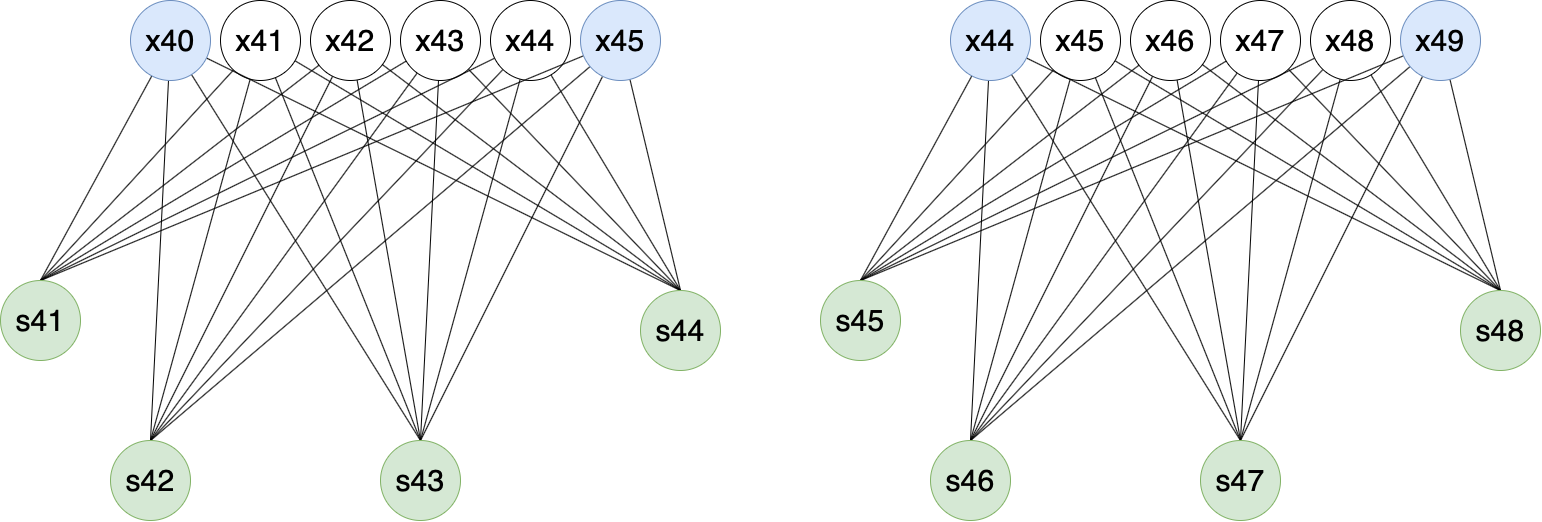
\includegraphics[scale=0.3]{Grafo_DES-expansion2.png}
    \caption{Graph edges for expansion function and $S$-box ($S_3$ and $S_4$) analysis, part 2}
    \label{fig:expansion2}
\end{figure}

\begin{figure}[h!]
    \centering
    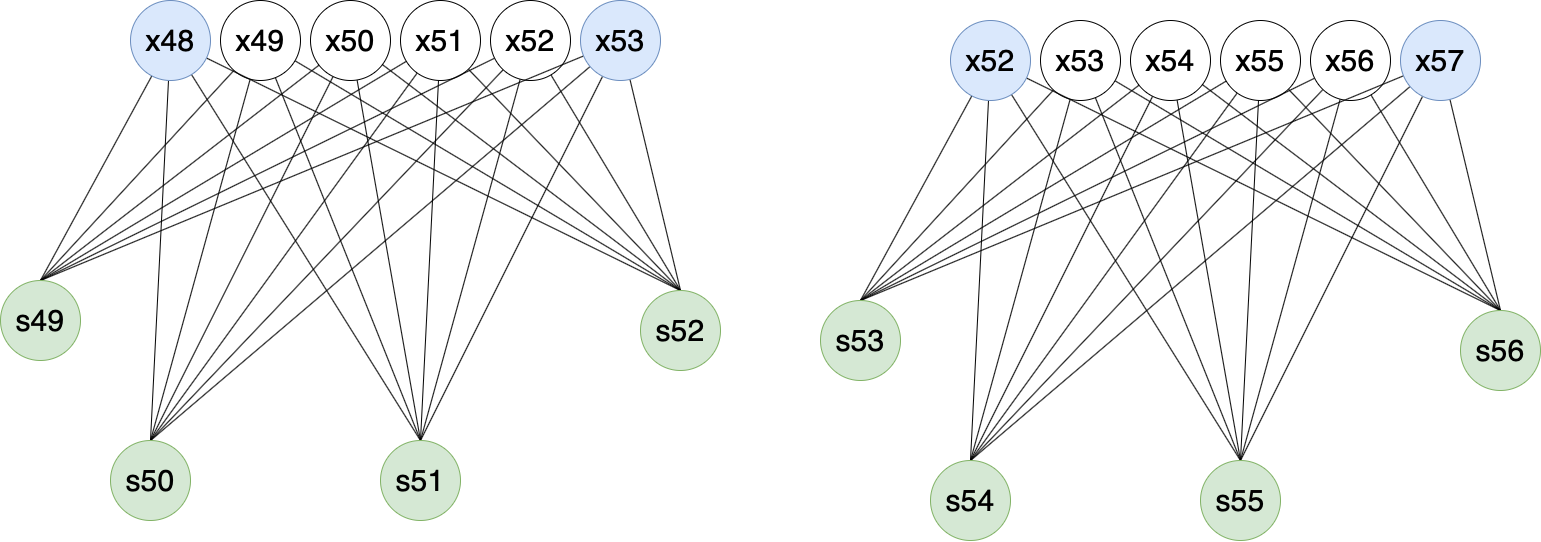
\includegraphics[scale=0.3]{Grafo_DES-expansion3.png}
    \caption{Graph edges for expansion function and $S$-box ($S_5$ and $S_6$) analysis, part 3}
    \label{fig:expansion3}
\end{figure}

\begin{figure}[h!]
    \centering
    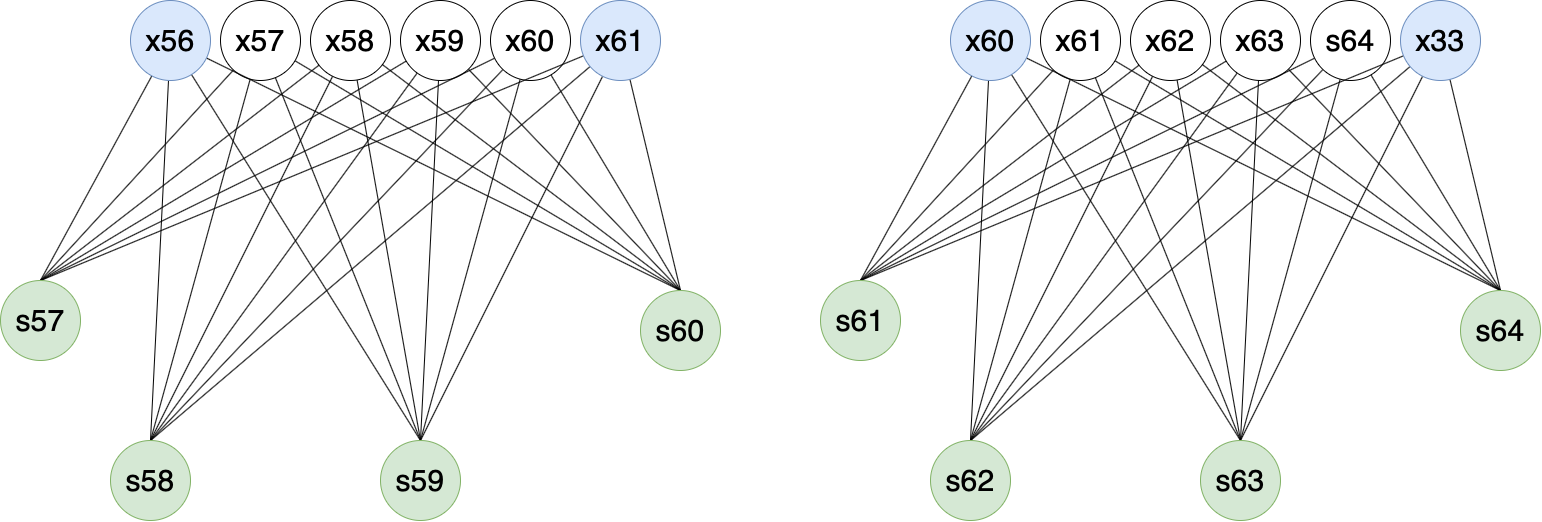
\includegraphics[scale=0.3]{Grafo_DES-expansion4.png}
    \caption{Graph edges for expansion function and $S$-box ($S_7$ and $S_8$) analysis, part 4}
    \label{fig:expansion4}
\end{figure}

\subsection{The permutation $P$}
After the $S$-boxes, the permutation $P$ is performed and this completes the $F$ function of DES. We thus need edges between $s_i^j$ bits ($S$-box results) and $x_i^1$ bits (the bits after the $F$ function has finally been completely applied to $R_0$ and the results have been incorporated to the round $1$ output).

What happens is, thus, that $x_{33}^1$ will actually depend on the sixteenth bit of the $S$-boxes output, which is $s_{48}^1$, due to the permutation $P$ (see Table \ref{tab:des-p}). In general, $x_i^j$ depends on $s_{P[i-32]+32}^j$. Figures \ref{fig:perm1} to \ref{fig:perm4} illustrate this.

\begin{table}[h!]
\centering
\begin{tabular}{|c|c|c|c|}
\hline
\multicolumn{4}{|c|}{P} \\ \hline
16   & 7    & 20  & 21  \\ \hline
29   & 12   & 28  & 17  \\ \hline
1    & 15   & 23  & 26  \\ \hline
5    & 18   & 31  & 10  \\ \hline
2    & 8    & 24  & 14  \\ \hline
32   & 27   & 3   & 9   \\ \hline
19   & 13   & 30  & 6   \\ \hline
22   & 11   & 4   & 25  \\ \hline
\end{tabular}
\caption{The $P$ permutation}
\label{tab:des-p}
\end{table}

\begin{figure}[h!]
    \centering
    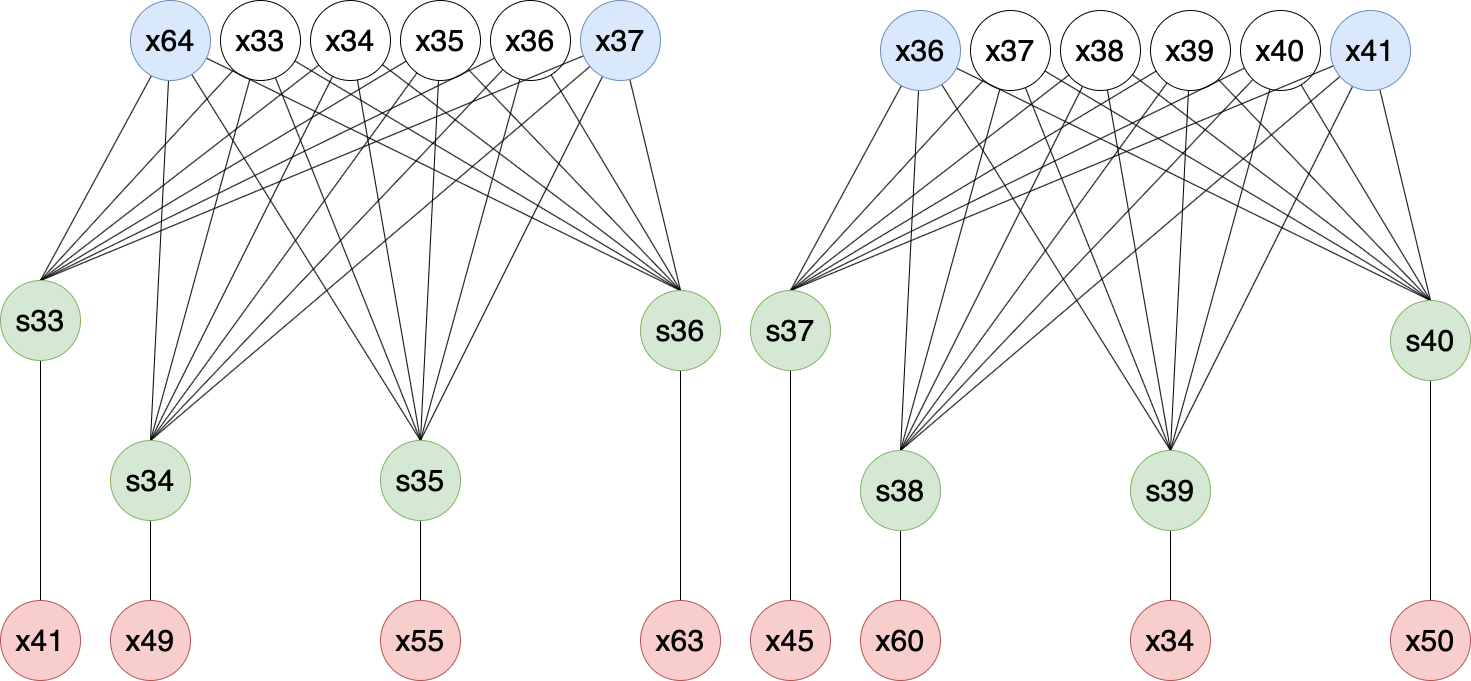
\includegraphics[scale=0.3]{Grafo_DES-p1.png}
    \caption{Graph edges for the $P$ permutation, part 1}
    \label{fig:perm1}
\end{figure}

\begin{figure}[h!]
    \centering
    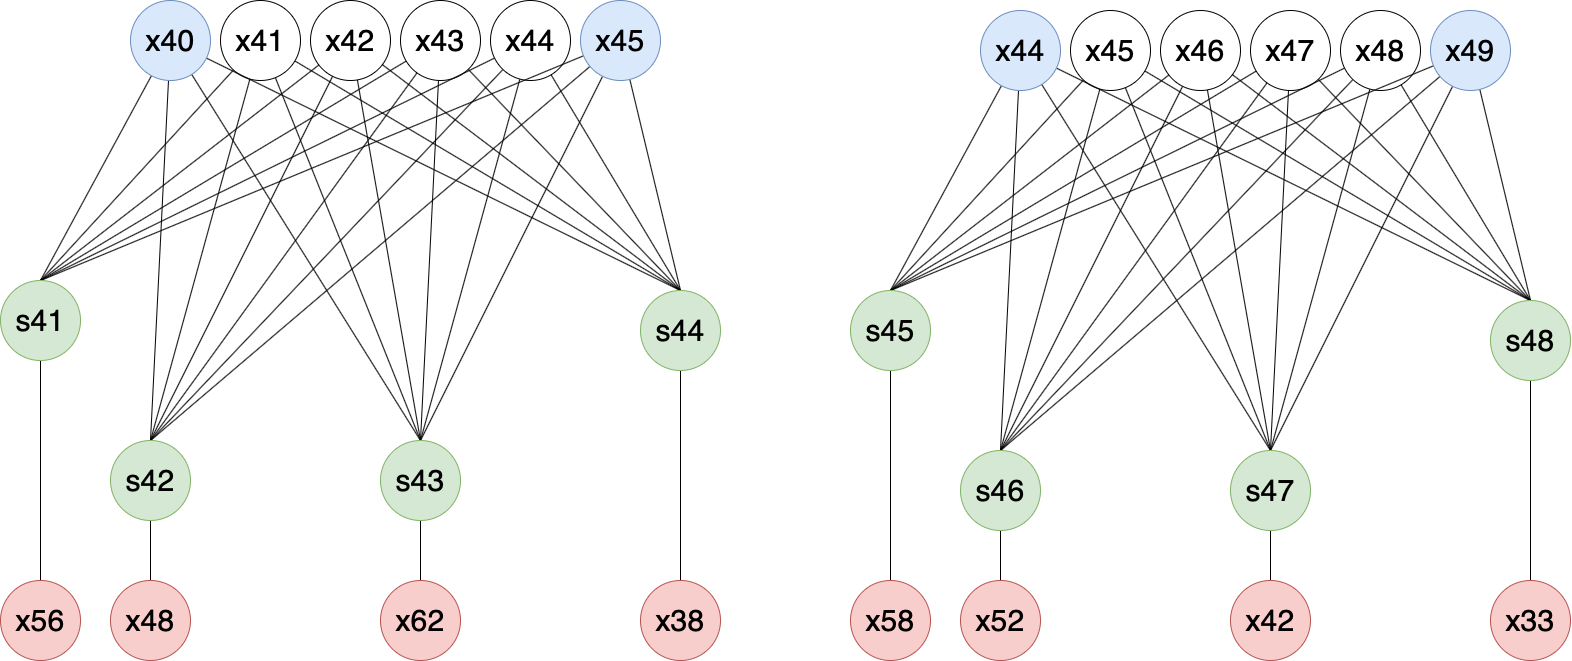
\includegraphics[scale=0.3]{Grafo_DES-p2.png}
    \caption{Graph edges for the $P$ permutation, part 2}
    \label{fig:perm2}
\end{figure}

\begin{figure}[h!]
    \centering
    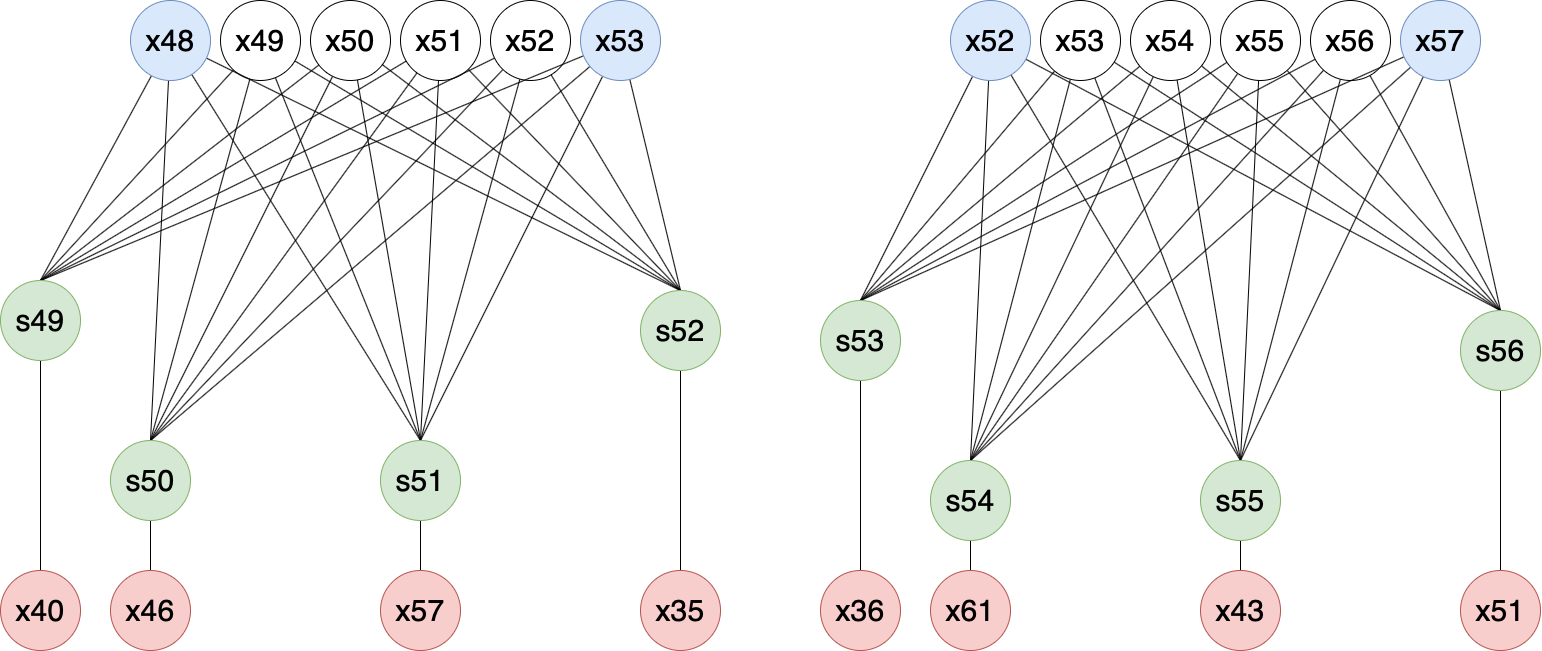
\includegraphics[scale=0.3]{Grafo_DES-p3.png}
    \caption{Graph edges for the $P$ permutation, part 3}
    \label{fig:perm3}
\end{figure}

\begin{figure}[h!]
    \centering
    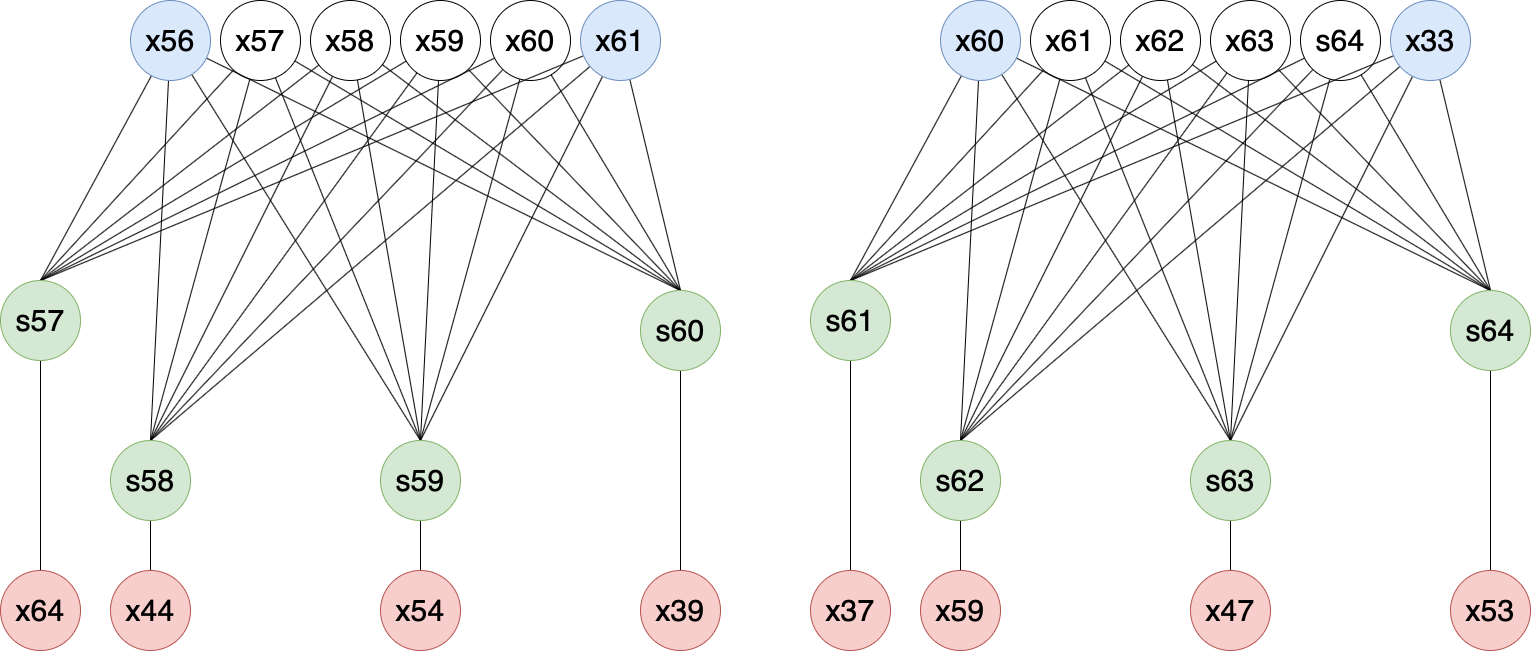
\includegraphics[scale=0.3]{Grafo_DES-p4.png}
    \caption{Graph edges for the $P$ permutation, part 4}
    \label{fig:perm4}
\end{figure}

Once edges between $x_i^1$ nodes and $s_i^1$ nodes have been created, the effect of $F$ has been completely tracked with regards to diffusion on the first round of DES. A state bit $x_i^1$ is dependent on a plaintext bit $x_k^0$ if there is a path from $x_i^1$ to $x_k^0$ in the graph.

\begin{figure}[h!]
    \centering
    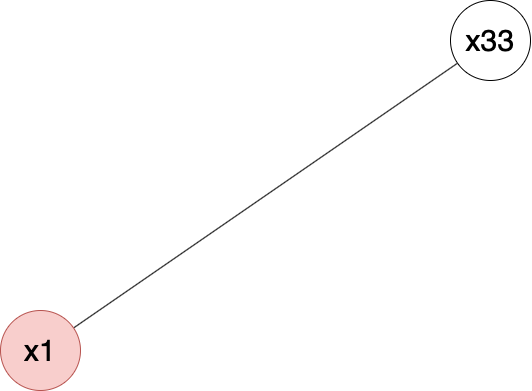
\includegraphics[scale=0.3]{Grafo_DES-node-example2.png}
    \caption{Graph paths for $x_1^1$}
    \label{fig:x1example}
\end{figure}

\begin{figure}[h!]
    \centering
    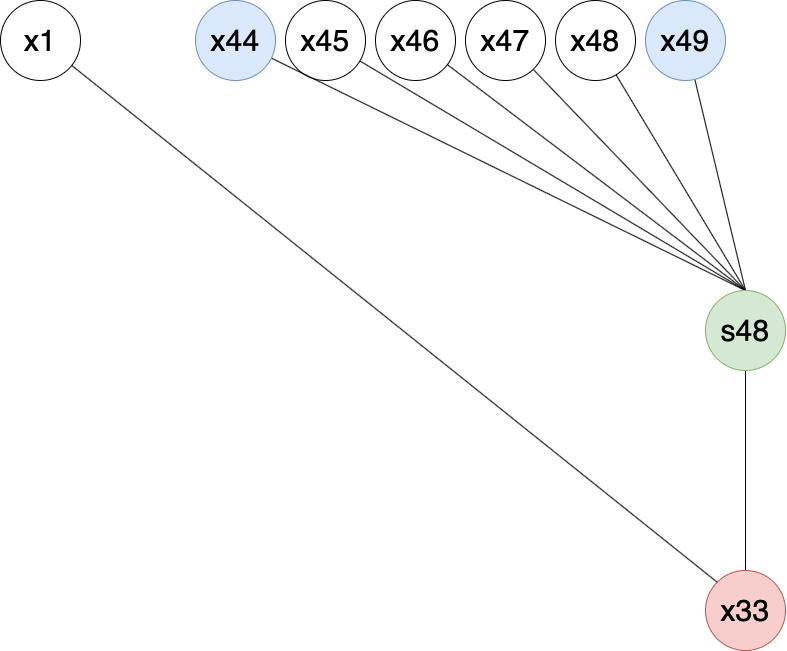
\includegraphics[scale=0.3]{Grafo_DES-node-example.png}
    \caption{Graph paths for $x_{33}^1$}
    \label{fig:x33example}
\end{figure}

\subsection{Facilitating path checks}\label{sec:graph-simplication}
Examples with all the paths for $x_1^1$ and $x_{33}^1$ are shown by Figures \ref{fig:x1example} and \ref{fig:x33example}, respectively. Note that $x_1^1$ depends only on $x_{33}^0$, because it has only been copied on the $L_1 = R_0$ step --- $F$ has not been applied to it yet --- while $x_{33}^1$ depends on 7 plaintext bits: $x_1$ due to the logical XOR with $L_0$, and the other six due to the application of $F$.

The intermediate nodes $s_i^j$, which represent $S$-Box outputs (green nodes in the figures) are not truly necessary for the implementation, since we are interested only in monitoring plaintext diffusion, although they help us explain the process. We can thus, when implementing this approach, create edges in the graph in the following way: \emph{if there exists a path from $x_i^1$ to $x_k^0$, create an edge directly between them, because, with an adjacency matrix representation, we can check if there is an edge between two nodes in $O(1)$ time} --- and thus we can immediately assess whether $x_i^1$ depends on $x_k^0$.

\subsection{Expanding the analysis to all rounds with adjacency matrices}
Graphs can be represented through adjacency lists or through an adjacency matrix. With an adjacency matrix representation, it is possible to make use of matrix exponentiation to expand the analysis towards all $16$ rounds of DES, having computed the adjacency matrix which represents the diffusion for round $1$. 

We start by representing the dependencies of the first round with an adjacency matrix. A $64\times64$ adjacency matrix $A$ can be built such that $A[r][c] = 1$ if the $c$-th bit after round $1$ depends on the $r$-th bit of plaintext, and $0$ otherwise. $A^1$ represents diffusion at round $1$, $A^2$ represents diffusion at round $2$, and so forth. When all elements of $A^p$ are nonzero, it means that complete plaintext diffusion is achieved at round $p$ of DES.

\subsection{Plaintext diffusion results}\label{sec:figs}

With this method, we observed that $A^5$ does not contain zeroes, thus DES achieves complete diffusion by the end of round $5$, since each state bit depends on all the plaintext bits.

It is relevant to note that elements greater than $1$ will appear in $A^p$ when $p > 1$, because of the sums that occur in the product. Therefore, in our implementation, elements greater than zero (not necessarily equal to $1$) indicate dependence between bits, while elements equal to zero indicate no dependence between the corresponding bits.

If one wishes matrices with only zeroes ore ones, the addition of elements can be replaced by a logical OR operation --- if $A^p[i][j] = 1$, $A^q[i][j]$ should be $1$ for all $q > p$, because a dependence between plaintext and state bits should not disappear once it has appeared in a certain round.

Unfortunately, the obtained 64x64 matrices are too large to be completely displayed in this document with good image quality. We make them available as \texttt{.csv} files at \textcolor{red}{add GitHub link here in the future}, together with our code. Figures \ref{fig:desdif1} to \ref{fig:desdif5} show a graphic representation of them. Black dots indicate state bits which depend on plaintext bits, and white regions are regions in which diffusion has not yet occurred.

\begin{figure}[H]
    \centering
    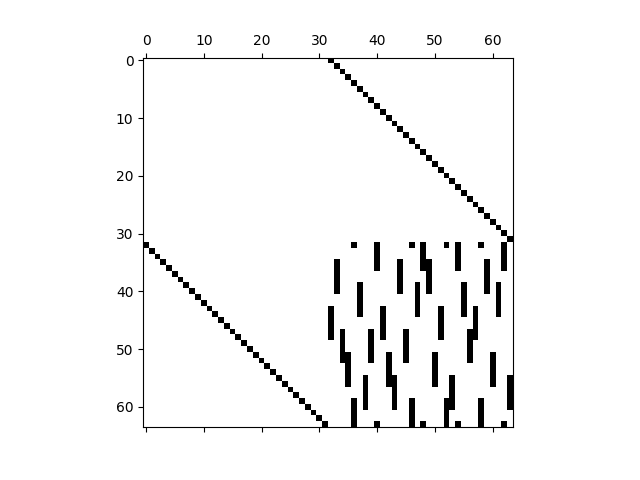
\includegraphics[scale=0.7]{sparse_des_difusao_iteracao_1.png}
    \caption{DES diffusion at round $1$}
    \label{fig:desdif1}
\end{figure}
\begin{figure}[H]
    \centering
    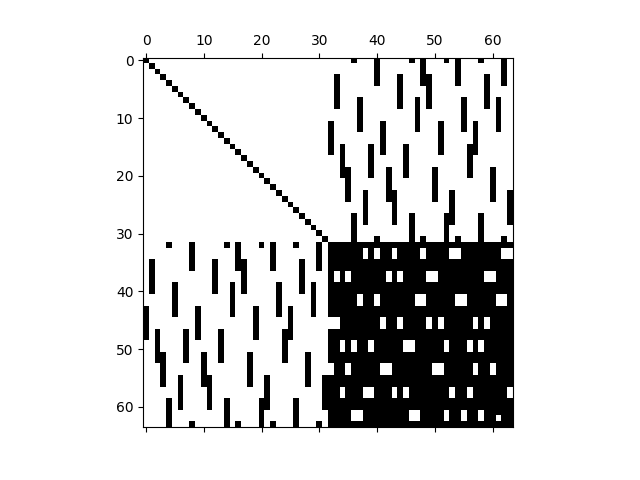
\includegraphics[scale=0.7]{sparse_des_difusao_iteracao_2.png}
    \caption{DES diffusion at round $2$}
    \label{fig:desdif2}
\end{figure}
\begin{figure}[H]
    \centering
    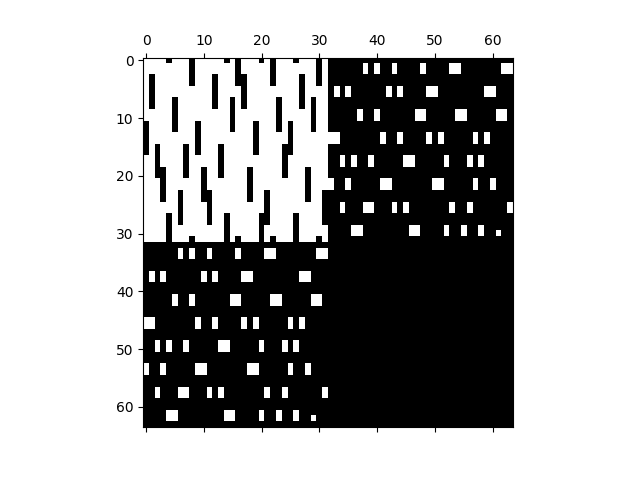
\includegraphics[scale=0.7]{sparse_des_difusao_iteracao_3.png}
    \caption{DES diffusion at round $3$}
    \label{fig:desdif3}
\end{figure}
\begin{figure}[H]
    \centering
    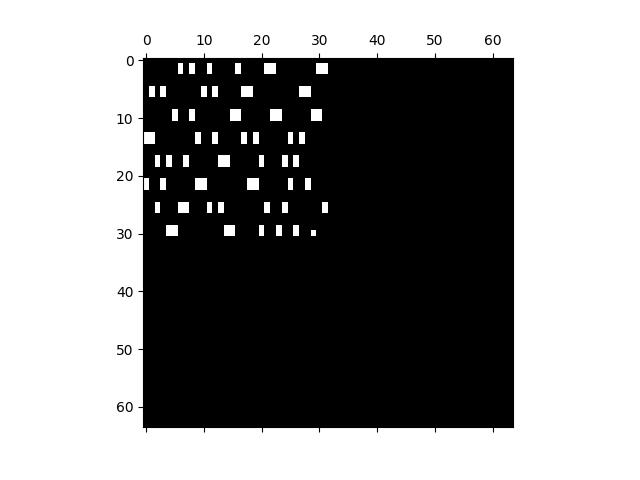
\includegraphics[scale=0.7]{sparse_des_difusao_iteracao_4.png}
    \caption{DES diffusion at round $4$}
    \label{fig:desdif4}
\end{figure}
\begin{figure}[H]
    \centering
    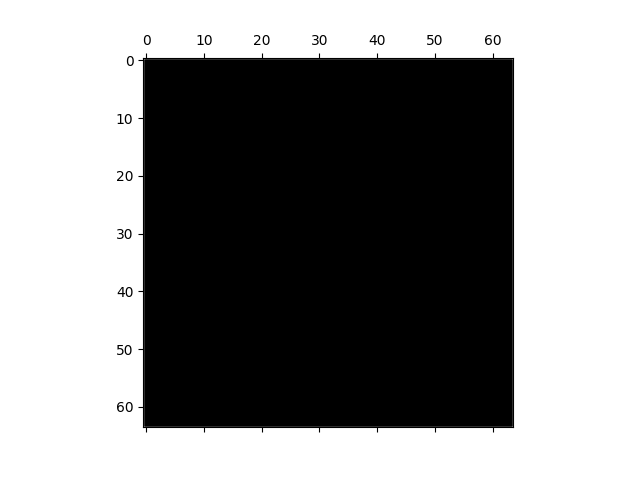
\includegraphics[scale=0.7]{sparse_des_difusao_iteracao_5.png}
    \caption{DES diffusion at round $5$ (finally complete!)}
    \label{fig:desdif5}
\end{figure}

\section{Key diffusion}\label{sec:key-diff}
In order to analyse key diffusion within DES, the process is analogous to the one employed for the plaintext. We model the problem as a graph, create nodes to represent the variables, and add edges to track dependence between them. However, at each round a different subkey is used. Furthermore, the subkeys are smaller than the state (they have 48 bits whilst the state contains 64 bits), and they are input to DES differently. Because of that, we cannot use matrix exponentiation to expand the analysis to all rounds once we have a matrix to represent the dependencies related to round 1. Therefore, for the key diffusion analysis, we have implemented the graph as an adjacency list.

Also, since each subkey is derived from the master key through the key scheduling process, a thorough understanding of the key scheduling routine is required. Algorithm \ref{alg:des-key-schedule} describes the key scheduling process, also known as \emph{key expansion} or \emph{key derivation}.

\begin{algorithm}[H]
\caption{DES key schedule}
\label{alg:des-key-schedule}
\begin{algorithmic}[1]
    \Require A 64-bit key $K = k_1k_2...k_{63}k_{64}$
    \Ensure Sixteen 48-bit subkeys $K_1, K_2, ..., K_{16}$
    \State Define $v_i, 1 \leq i \leq 16$, as follows: $v_i = 1$ for $i \in \{1, 2, 9, 16\}$, $v_i = 2$ otherwise
    
    \State $T \gets PC1(K)$
    \Comment PC1 is a permutation
    \State Represent $T$ as two 28-bit halves $C_0$ and $D_0$, such that $C_0 = k_{57}k_{49}...k_{36}$ and $D_0 = k_{63}k_{55}...k_{4}$
    \For{$i = 1, ..., 16$}
        \State $C_i \gets C_{i-1} << v_i$
        \Comment Here $<<$ denotes a left circular shift
        \State $D_i \gets D_{i-1} << v_i$
        \State Represent the concatenation of $C_i$ and $D_i$ as $B = b_1b_2...b_{56}$
        \State $K_i \gets PC2(B)$
        \Comment PC2 is a permutation
    \EndFor

\end{algorithmic}
\end{algorithm}

The permutations $PC1$ and $PC2$ mentioned on Algorithm \ref{alg:des-key-schedule} are shown by tables \ref{tab:pc1} and \ref{tab:pc2}, respectively.

\begin{table}[H]
\centering
\begin{tabular}{|c|c|c|c|c|c|c|}
\hline
\multicolumn{7}{|c|}{PC1}                                         \\ \hline
57      & 49      & 41      & 33      & 25      & 17     & 9      \\ \hline
1       & 58      & 50      & 42      & 34      & 26     & 18     \\ \hline
10      & 2       & 59      & 51      & 43      & 35     & 27     \\ \hline
19      & 11      & 3       & 60      & 52      & 44     & 36     \\ \hline
\multicolumn{7}{|c|}{above for $C_i$, below for $D_i$} \\ \hline
63      & 55      & 47      & 39      & 31      & 23     & 15     \\ \hline
7       & 62      & 54      & 46      & 38      & 30     & 22     \\ \hline
14      & 6       & 61      & 53      & 45      & 37     & 29     \\ \hline
21      & 13      & 5       & 28      & 20      & 12     & 4      \\ \hline
\end{tabular}
\caption{The PC1 permutation}
\label{tab:pc1}
\end{table}

\begin{table}[H]
\centering
\begin{tabular}{|c|c|c|c|c|c|c|}
\hline
\multicolumn{7}{|c|}{PC2}        \\ \hline
14 & 17 & 11 & 24 & 1  & 5  & 9  \\ \hline
3  & 28 & 15 & 6  & 21 & 10 & 18 \\ \hline
23 & 19 & 12 & 4  & 26 & 8  & 27 \\ \hline
16 & 7  & 27 & 20 & 13 & 2  & 36 \\ \hline
41 & 52 & 31 & 37 & 47 & 55 & 15 \\ \hline
30 & 40 & 51 & 45 & 33 & 48 & 22 \\ \hline
44 & 49 & 39 & 56 & 34 & 53 & 29 \\ \hline
46 & 42 & 50 & 36 & 29 & 32 & 4  \\ \hline
\end{tabular}
\caption{The PC2 permutation}
\label{tab:pc2}
\end{table}

The input to the algorithm is the original key, i.e master key, which comprises 64 bits. The algorithm outputs sixteen 48-bit subkeys, which are to be used in each of the DES sixteen rounds, respectively. $K_1$ is used at round 1, $K_2$ at round 2, and so forth. Subkeys must not be repeated in different rounds --- once they have been used in their corresponding round, they are no longer used.

The first step is to permute the master key, using $PC1$. Then, the result of the permutation is split into 28-bit halves, here denoted as $C_0$ and $D_0$. After that, the $C_i$ and $D_i$ for each round $i$, $1 \leq i \leq 16$, are generated by means of circular left shifts. The left shift depends on the values of the $v_i$ ($1$ for rounds $1, 2, 9$ and $16$, $2$ otherwise). Once $C_i$ and $D_i$ have been generated, their concatenation, denoted by $B$, is permuted, this time with permutation $PC2$, and the result of this permutation is the subkey $K_i$ of round $i$.

\subsection{Modeling key diffusion as a graph}
In order to track the diffusion of the key, intermediate nodes are helpful once again. Let $x^r_l$ be a node that represents the $l$-th bit of the state at round $r$, $s^r_j$ be a node that represents the $j$-th bit of an $S$-box output for round $r$, and $K_{r,z}$ be a node that represents the $z$-th bit of a subkey used in round $r$.

First, consider the $j$-th bit of the output of an $S$-box of the first round, hence a node $s^1_j$. In our previous analysis, which considered only plaintext, we create and edge from $s^1_j$ to $x^0_l$. However, in truth, the input to an $S$-box is not composed by state bits only --- it is \emph{the logical XOR of six state bits and six round key bits}. Therefore, if a round key bit $K_{1,z}$ is XORed to $x^0_l$ in DES, there should also be an edge between $s^1_j$ and $K_{1,z}$ to track this dependence. Thus a state bit of round 1, e.g $x^1_w$ which happens to depend on the $S$-box output $s^1_j$, will have a path towards $K_{1,z}$ as well.

For the other rounds, such as round 2, the same logic is applied. The intermediate nodes which represent $S$-box outputs should have edges towards the nodes of the form $K_{2,v}$, which represent bits of the second subkey, i.e the key used for round 2.

In order to track the dependence directly to the master key bits, the nodes of the form $K_{r,z}$ have edges towards nodes of the form $k_p$, where $k_p$ represents the $p$-th bit of the master key. A state bit thus depends on a master key bit if there is a path between them. Figure \ref{fig:keydiff} illustrates the graph edges for the state bit $x^1_{33}$. 

\begin{figure}[H]
    \centering
    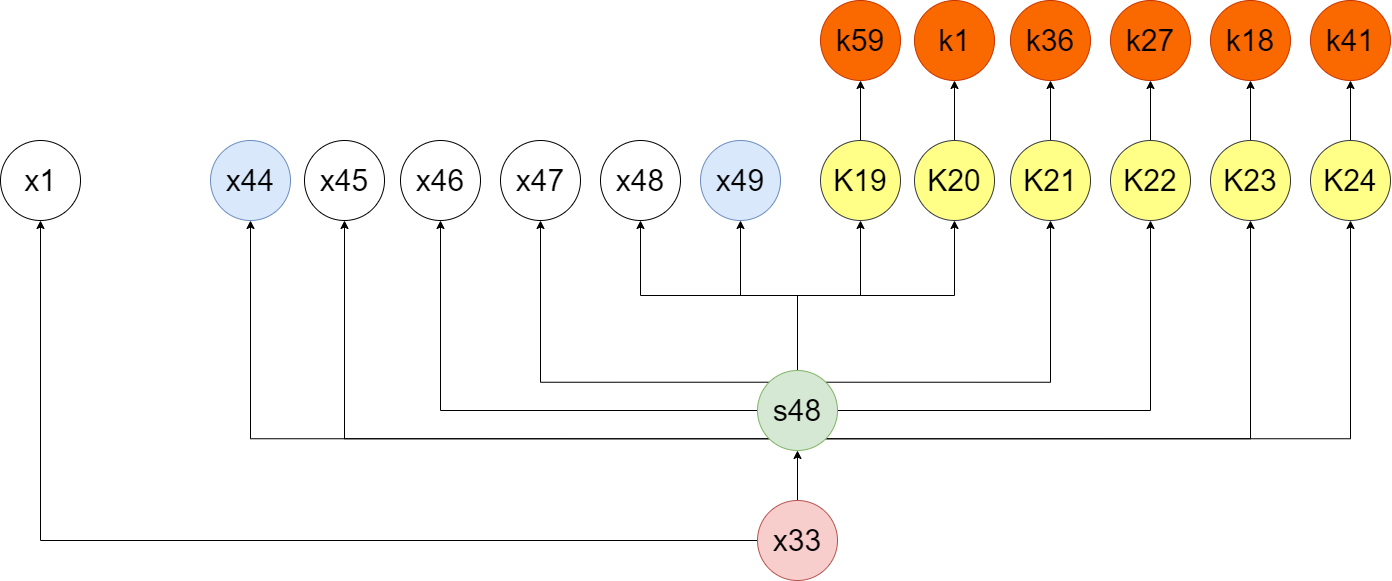
\includegraphics[scale=0.25]{figura_key_diffusion.png}
    \caption{An example of key diffusion dependence tracking. White nodes and blue nodes refer to plaintext bits, the green node refers to the $S$-box output, yellow nodes refer to the subkey, orange nodes refer to the master key, and the red node refers to a round 1 state bit.}
    \label{fig:keydiff}
\end{figure}

To obtain the edges between subkey nodes and master key nodes, we follow the key derivation process and make use of intermediate nodes. In our implementation, we created nodes for each step of the key derivation: nodes for bits of $T$, bits of $C_i$ and $D_i$, of $B$ and, finally, of the master key $k$. And, to easily find the dependence, when there is a path from a node $X$ to a node $Y$, we add an edge directly from $X$ to $Y$, as described in Section \ref{sec:graph-simplication}. In this way, a round key bit of the type $K_i$ is directly mapped to a master key bit of the type $k$ and assessing whether the dependency holds no longer requires checking the existence of a path from in the graph, only the existence of an edge.

\subsection{Key diffusion results}
With this method, we could determine that DES also achieves complete key diffusion \emph{by the end of the fifth round}. Another fact is that, if we start e.g from round 2, complete key diffusion will be achieved by the end of round 6. If we start from round 3, it will be achieved by the end of round 7, and so forth. In other words, it does not matter which round we start from, the key will have been completely diffused after 5 rounds.

It is relevant to note that, from the 64 bits of the master key, 8 are deemed parity bits, and they are not used, i.e diffused. Thus the complete diffusion is achieved when each state bit depends on 56 master key bits. Table \ref{tab:key-dif-des} shows the key diffusion for the first 5 rounds of DES, with minimum key diffusion referring to a state bit which depends on the smallest amount of master key bits and maximum key diffusion referring to a state bit which depends on the largest amount of master key bits.

\begin{table}[H]
\centering
\begin{tabular}{|c|c|c|}
\hline
\textbf{Round} & \textbf{Minimum key diffusion} & \textbf{Maximum key diffusion} \\ \hline
1              & 6                              & 6                              \\ \hline
2              & 6                              & 39                             \\ \hline
3              & 36                             & 56                             \\ \hline
4              & 52                             & 56                             \\ \hline
5              & 56                             & 56                             \\ \hline
\end{tabular}
\caption{Key diffusion along the first five DES rounds}
\label{tab:key-dif-des}
\end{table}

At round $5$, the minimum key diffusion is $56$, thus all the key bits have spread their influence to all the state bits, and complete diffusion has been achieved.

\section{Implementation remarks and computational complexity}\label{sec:complexity}

For the plaintext diffusion analysis, the computational complexity entails the construction of a $64\times64$ matrix $A$ representing the dependencies and, then, matrix exponentiation in order to obtain $A^5$. Due to the small size of the matrix and the small exponent, the computational cost of this method is negligible.

For the key diffusion analysis, the adjacency-list construction can also be done with negligible computational cost, since only a constant amount of edges must be created due to the structure of the DES cipher. Section \ref{sec:upper-bound} generalizes the analysis and provides upper bounds for the computational complexity of our approach.

\subsection{Asymptotic complexity and an upper bound}\label{sec:upper-bound}

\subsubsection{Upper bound for plaintext diffusion analysis}

In general, constructing an adjacency matrix to track diffusion from the plaintext towards the first round of a block cipher of block size $n_b$, not necessarily a Feistel Network, and not necessarily similar to DES, would require $O(n_b)$ time. For each round $1$ output bit, we need to create the correct edges (assuming edges can be created in constant time). In the worst case, if all round $1$ bits have edges towards all plaintext bits, $n_b^2$ edges would have to be created. Therefore, the worst case run time is $O(n_b^2)$ and the average case run time is $O(n_b)$ to construct the matrix.

A naive matrix multiplication algorithm requires $O(n^3)$ time to multiply two $n \times n$ matrices. If we were to apply this method to a cipher of block size $n_b$ and $n_r$ rounds, assuming we wish to obtain all matrices for all rounds, the complexity would be $O(n_r \cdot n_b^3)$, with a naive exponentiation algorithm that required $n_r$ multiplications to obtain $A^{n_r}$. Matrix multiplication/exponentiation can be optimized e.g by means of Strassen's algorithm (see \cite{Cormen2009}) and many other approaches, and optimizing the implementation would be relevant when analysing ciphers with large $n_b$ and/or $n_r$ that made a naive implementation unpractical, but it is not the case for DES (and it would probably not be for other ciphers, sinze $n_r$ and $n_b$ are usually fixed and small).

Since constructing the matrix requires $O(n_b^2)$ time and the exponentiation requires $O(n_r \cdot n_b^3)$ time, the asymptotic complexity is $O(n_r \cdot n_b^3)$. However, since $n_r$ and $n_b$ are small and fixed, the practical run time is actually constant.

\subsubsection{Upper bound for key diffusion analysis}

For an $n_r$-round block cipher with $n_{sk}$-bit subkeys and block size $n_b$, the adequate edges must be created between each of the $n_{sk}$ bits and the $n_b$ round output bits. In the worst case, $n_b \cdot n_{sk}$ edges must be created at each round, if each round output bit depends on all the subkey bits. Therefore, the run time for this step is $O(n_r \cdot n_b \cdot n_{sk})$. 

However, there must be edges mapping from the subkey bits to the $n_k$ master key bits, and directly from the round output bits as well, to facilitate the dependency check. Therefore, $2 \cdot n_k \cdot n_{sk}$ more edges would be required, for each round, in the worst case (worst case = each bit of the subkey depends on all bits of the master key).

The asymptotic run time, considering edges can be created in constant time is thus $O(n_r \cdot n_k \cdot n_{sk} + n_r \cdot n_b \cdot n_{sk})$. However, as is the case of $n_b$ and $n_r$, $n_k$ and $n_{sk}$ are also fixed and small for most ciphers, which leads to constant time in practice.

\section{Conclusions and future work}
In this chapter, we analyzed the DES cipher with respect to plaintext diffusion and key diffusion. For this purpose, we model the DES cipher as a graph, with vertices for each state, plaintext and key bit, among other intermediate vertices to facilitate the comprehension of the process.

We show that DES achieves both complete plaintext and key diffusion by the end of the $5$-th round. For the plaintext diffusion analysis, we use the adjacency matrix representation of the graph and take advantage of matrix exponentiation. For the key diffusion analysis, we used the adjacency-list representation of the graph.

The approaches presented in this chapter have negligible computational cost, as argued in Section \ref{sec:complexity}, and thus they might provide an interesting method for diffusion analysis of other ciphers and cryptographic primitives. Furthermore, this chapter is limited to analysing the DES cipher. Other ciphers could be analyzed with this method, as well as hash functions and other cryptographic algorithms.

In Section \ref{sec:figs}, we mention that values greater than $1$ appear in the matrices because of the sums that occur in the exponentiation process. It could be interesting to assess whether they provide further information about the DES cipher diffusion.

Finally, the graph shows in detail all the dependencies between plaintext/key and round output bits. Attempts at different visual representations of the DES graph other than the one provided in Section \ref{sec:figs} would be interesting.

It is also worth investigating the application of other graph related concepts and algorithms, and whether they would allow us to obtain significant information regarding cryptographic algorithms modeled as graphs. In this chapter, we restrict to the construction of adjacency matrices and lists, but graphs have several other concepts that could be explored (e.g shortest paths, edge weights, among others).

\bibliographystyle{plain}
\bibliography{refs}
\end{document}
